% =====================================================================
%  section42_body.tex  ·  Section 4.2 — Concavity and Inflection Points
%  Seminar slides (Beamer).  Content = the handwritten notes exactly.
%  Do not compile this file directly: compile section35_dark.tex or
%  section35_light.tex (each one only chooses the theme, then \input's this).
% =====================================================================
\documentclass[aspectratio=169,11pt]{beamer}
\usepackage{amsmath,amssymb}
\usepackage{array,adjustbox,varwidth,hyperref}
\usepackage{pgfplots}\pgfplotsset{compat=1.17}
\usetikzlibrary{arrows.meta}
\usefonttheme[onlymath]{serif}       % math in Computer Modern, as in the video
\setbeamertemplate{navigation symbols}{}

% ---------------------------------------------------------------- palette
\ifdefined\usedark
  \definecolor{bg}{HTML}{0E1626}   \definecolor{ink}{HTML}{F4EFE6}
  \definecolor{muted}{HTML}{8D99AE}\definecolor{gold}{HTML}{E8C27A}
  \definecolor{teal}{HTML}{5FB3A8} \definecolor{card}{HTML}{162238}
  \definecolor{edge}{HTML}{2B3A55} \definecolor{dimc}{HTML}{5C6A84}
\else
  \definecolor{bg}{HTML}{FBFAF6}   \definecolor{ink}{HTML}{1B2333}
  \definecolor{muted}{HTML}{6B7487}\definecolor{gold}{HTML}{A8781F}
  \definecolor{teal}{HTML}{2E7D73} \definecolor{card}{HTML}{F1EEE6}
  \definecolor{edge}{HTML}{D9D3C5} \definecolor{dimc}{HTML}{A9AFBC}
\fi

\setbeamercolor{background canvas}{bg=bg}
\setbeamercolor{normal text}{fg=ink,bg=bg}
\setbeamercolor{frametitle}{fg=ink}
\setbeamercolor{itemize item}{fg=gold}
\setbeamercolor{block title}{fg=gold,bg=card}
\setbeamercolor{block body}{fg=ink,bg=card}
\setbeamertemplate{itemize item}{\raisebox{0.15ex}{\color{gold}$\bullet$}}

% ---------------------------------------------------------------- frame title + footline
\setbeamertemplate{frametitle}{%
  \vspace*{0.18cm}\usebeamerfont{frametitle}\bfseries\insertframetitle\par
  \vspace{-0.05cm}{\color{gold}\rule{1.4cm}{1.6pt}}\par\vspace{-0.1cm}}
\setbeamerfont{frametitle}{size=\Large}
\setbeamertemplate{footline}{%
  \leavevmode\hbox to\paperwidth{\hspace{0.5cm}%
  {\color{muted}\scriptsize Faculty Seminar \;$\cdot$\; Calculus \;$\cdot$\; Section 4.2}%
  \hfill{\color{muted}\scriptsize\insertframenumber\,/\,\inserttotalframenumber}\hspace{0.5cm}}\vspace{0.12cm}}

% ---------------------------------------------------------------- macros
\newcommand{\dydx}{{\color{gold}\frac{dy}{dx}}}
\newcommand{\yp}{{\color{gold}y'}}
\newcommand{\fpp}{{\color{gold}f''}}
% common pgfplots look
\pgfplotsset{sem/.style={axis lines=middle, axis line style={muted,-{Stealth[length=4pt]}},
  tick label style={font=\tiny,color=muted}, label style={font=\scriptsize,color=muted},
  xlabel={$x$}, ylabel={$y$}, every axis plot/.append style={line width=1.2pt}, clip=true}}
\newcommand{\ilink}[1]{\hfill\href{https://alostazy2k.github.io/seminars/4.2/concavity-explorer.html\##1}{\fcolorbox{gold}{bg}{\tiny\color{gold}\textnormal{Interactive}\,$\nearrow$}}}
\newlength{\textleft}\setlength{\textleft}{0.6cm}
\newcommand{\stmt}[1]{\vspace{0.1cm}{\small #1}\par\vspace{0.1cm}}
\newcommand{\sol}{{\color{gold}\small\bfseries\underline{Solution}}\par\vspace{-0.35cm}}
\newcommand{\sectag}[1]{\fcolorbox{gold}{bg}{\color{gold}\bfseries #1}\;}


\title{Concavity and Inflection Points}
\author{Dr.\ Wessam Gouda}
\date{}

\begin{document}

% ================================================================ title
{\setbeamertemplate{footline}{}
\begin{frame}[plain]
  \centering\vspace*{0.9cm}
  {\color{gold}\small\bfseries FACULTY SEMINAR \;$\cdot$\; CALCULUS}\par\vspace{0.3cm}
  {\color{muted}\large Section 4.2 \;$\cdot$\; Applications of Differentiation}\par\vspace{0.15cm}
  {\fontsize{28}{34}\selectfont\bfseries Concavity and Inflection Points}\par\vspace{0.25cm}
  {\color{gold}\rule{6cm}{1.2pt}}\par\vspace{0.3cm}
  {\Large$f''(x)>0\;\Rightarrow\;\smile\qquad f''(x)<0\;\Rightarrow\;\frown$}\par
  \vfill
  \begin{flushleft}\hspace*{0.4cm}{\color{gold}\vrule width 2pt}\hspace{0.25cm}%
  \begin{tabular}[b]{@{}l@{}}{\bfseries Dr.\ Wessam Gouda}\\{\color{muted}\scriptsize Department of Mathematics}\end{tabular}
  \end{flushleft}\vspace*{0.2cm}
\end{frame}}

% ================================================================ agenda
\begin{frame}{Agenda}
  \vspace{0.3cm}
  \begin{columns}[T]
  \begin{column}{0.47\textwidth}
    \begin{tabular}{@{}l@{\hspace{0.35cm}}l@{}}
      {\color{gold}\bfseries 01} & Learning Objectives\\[0.26cm]
      {\color{gold}\bfseries 02} & Concavity: definition \& test\\[0.26cm]
      {\color{gold}\bfseries 03} & Interactive: Concavity Explorer\\[0.26cm]
      {\color{gold}\bfseries 04} & Related Problem 1\\[0.26cm]
      {\color{gold}\bfseries 05} & Inflection points\\[0.26cm]
      {\color{gold}\bfseries 06} & Example 2
    \end{tabular}
  \end{column}
  \begin{column}{0.47\textwidth}
    \begin{tabular}{@{}l@{\hspace{0.35cm}}l@{}}
      {\color{gold}\bfseries 07} & Examples 3, 6, 8, 9\\[0.26cm]
      {\color{gold}\bfseries 08} & The Second Derivative Test\\[0.26cm]
      {\color{gold}\bfseries 09} & Example 10 (1)\\[0.26cm]
      {\color{gold}\bfseries 10} & Challenging Problems 5\\[0.26cm]
      {\color{gold}\bfseries 11} & Communicate with Mathematics 2
    \end{tabular}
  \end{column}
  \end{columns}
\end{frame}

% ================================================================ objectives
\begin{frame}{Learning Objectives}
  \vspace{0.3cm}
  At the end of this section, you should be able to:\par\vspace{0.35cm}
  \begin{itemize}\setlength{\itemsep}{0.4cm}
    \item<1-> Investigate additional features of graphs of functions, particularly concavity and points of inflection.
    \item<2-> Explore and analyze the concavity of graphs of functions using the methods of calculus.
    \item<3-> Identify and determine points of inflection of a function using calculus techniques.
  \end{itemize}
\end{frame}

% ================================================================ concavity idea
\begin{frame}[t]{Concavity \ilink{sin}}
  \small The first derivative is the slope of the tangent line; the \textbf{second derivative} describes how that slope changes --- the \emph{curvature} of the graph.\par
  \centering\vspace{0.1cm}
  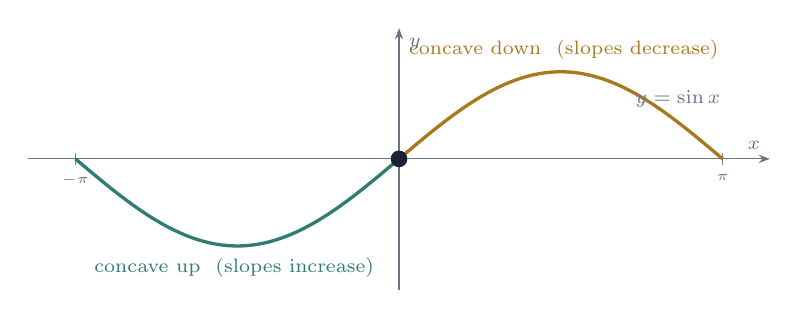
\begin{tikzpicture}\begin{axis}[sem,width=11cm,height=4.9cm,xmin=-3.6,xmax=3.6,ymin=-1.5,ymax=1.5,
      xtick={-3.1416,0,3.1416},xticklabels={$-\pi$,$0$,$\pi$},ytick=\empty]
    \addplot[teal,domain=-3.1416:0,samples=80]{sin(deg(x))};
    \addplot[gold,domain=0:3.1416,samples=80]{sin(deg(x))};
    \addplot[only marks,mark=*,mark size=2.4pt,ink] coordinates{(0,0)};
    \node[teal,font=\scriptsize] at (axis cs:-1.6,-1.25){concave up \ (slopes increase)};
    \node[gold,font=\scriptsize] at (axis cs:1.6,1.25){concave down \ (slopes decrease)};
    \node[muted,font=\scriptsize,anchor=north west] at (axis cs:2.2,0.9){$y=\sin x$};
  \end{axis}\end{tikzpicture}\par
  {\scriptsize\color{muted} Concave up: the graph lies \textbf{above} its tangent lines. \quad Concave down: the graph lies \textbf{below} its tangent lines.}
\end{frame}

% ================================================================ def 4.2.1 + test
\begin{frame}[t]{Definition 4.2.1 \;\&\; Theorem 4.2.1}
  \begin{block}{Definition 4.2.1 \ (Concave Up or Concave Down)}
    Let $f$ be a differentiable function on an open interval $I$. Then
    \begin{enumerate}
      \item $f$ is said to be \textbf{concave up} on $I$ if $f'$ is increasing on $I$.
      \item $f$ is said to be \textbf{concave down} on $I$ if $f'$ is decreasing on $I$.
    \end{enumerate}
  \end{block}
  \uncover<2->{%
  \begin{block}{Theorem 4.2.1 \ (Concavity Test)}
    Suppose $f''(x)$ exists on an open interval $I$.
    \begin{enumerate}
      \item If $f''(x)>0$ on $I$, then $f$ is concave up on $I$.
      \item If $f''(x)<0$ on $I$, then $f$ is concave down on $I$.
    \end{enumerate}
  \end{block}}
\end{frame}

% ================================================================ explorer
\begin{frame}[t]{Interactive: Concavity Explorer}
  \vspace{0.2cm}
  \begin{columns}[T]
  \begin{column}{0.55\textwidth}\small
    Drag a point along the curve and watch:
    \begin{itemize}\setlength{\itemsep}{0.15cm}
      \item the tangent line and its slope $f'(x)$,
      \item the sign of $f''(x)$,
      \item the curve coloured \textcolor{teal}{concave up} / \textcolor{gold}{concave down},
      \item the inflection points marked.
    \end{itemize}
    Functions: the examples of this seminar.
  \end{column}
  \begin{column}{0.4\textwidth}\centering
    \vspace{0.4cm}
    \href{https://alostazy2k.github.io/seminars/4.2/concavity-explorer.html}{\fcolorbox{gold}{card}{\parbox{4.6cm}{\centering\vspace{0.15cm}{\color{gold}\bfseries Open the\\Concavity Explorer}\vspace{0.15cm}}}}\par\vspace{0.3cm}
    {\tiny\color{muted}\url{https://alostazy2k.github.io/seminars/4.2/concavity-explorer.html}}\par\vspace{0.25cm}
    {\scriptsize\href{run:concavity-explorer.html}{\color{teal}\underline{offline copy (same folder as this PDF)}}}
  \end{column}
  \end{columns}
\end{frame}

% ================================================================ related problem 1
\begin{frame}[t]{Related Problem 1 \ilink{rp1}}
  \stmt{Use the graph of $y=f'(x)$, given in the figure, to find the following: \ 1.\ The intervals on which $f$ is concave up. \ 2.\ The intervals on which $f$ is concave down.}
  \begin{columns}[T]
  \begin{column}{0.52\textwidth}\centering
    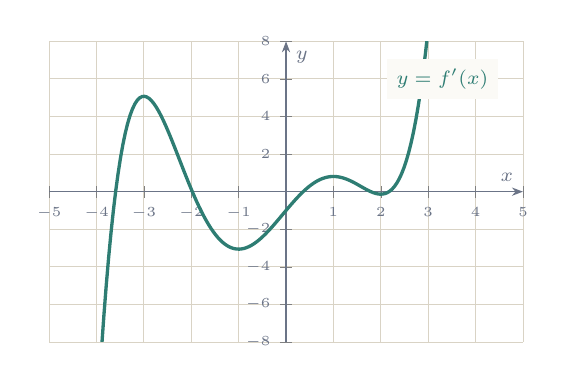
\begin{tikzpicture}\begin{axis}[sem,width=7.6cm,height=5.4cm,xmin=-5,xmax=5,ymin=-8,ymax=8,
        xtick={-5,-4,-3,-2,-1,1,2,3,4,5},ytick={-8,-6,-4,-2,2,4,6,8},grid=both,grid style={edge,line width=0.3pt}]
      \addplot[teal,domain=-5:5,samples=200]{0.5*(x^5/5+x^4/4-7*x^3/3-x^2/2+6*x)-1};
      \node[teal,font=\scriptsize,fill=bg] at (axis cs:3.3,6){$y=f'(x)$};
    \end{axis}\end{tikzpicture}\par
    {\tiny\color{muted} graph redrawn with the same turning points as Figure 4.2.4}
  \end{column}
  \begin{column}{0.44\textwidth}\small
    {\color{gold}\bfseries\underline{Answer}}\par\vspace{0.25cm}
    \uncover<2->{$f'$ increasing on $(-\infty,-3),\,(-1,1),\,(2,\infty)$\par\vspace{0.1cm}
    $\Rightarrow$ \textbf{1.\ Concave up on} $(-\infty,-3),\,(-1,1),\,(2,\infty)$\par\vspace{0.35cm}}
    \uncover<3->{$f'$ decreasing on $(-3,-1),\,(1,2)$\par\vspace{0.1cm}
    $\Rightarrow$ \textbf{2.\ Concave down on} $(-3,-1),\,(1,2)$}
  \end{column}
  \end{columns}
\end{frame}

% ================================================================ inflection
\begin{frame}[t]{Definition 4.2.2 \;\&\; Theorem 4.2.2}
  \begin{block}{Definition 4.2.2 \ (Inflection Point)}
    Let $f$ be a continuous function on an open interval $I$ and $x_0\in I$. Then the point $(x_0,f(x_0))$ is said to be an \textbf{inflection point} if $f(x)$ changes its concavity (upward to downward or downward to upward) around $x_0$.
  \end{block}
  \uncover<2->{%
  \begin{block}{Theorem 4.2.2 \ (Points of Inflection)}
    Let $(c,f(c))$ be a point of inflection of the graph of the function $f$. Then, either $f''(c)=0$, or $f''(c)$ does not exist.
  \end{block}}
  \uncover<3->{\centering\vspace{0.05cm}
  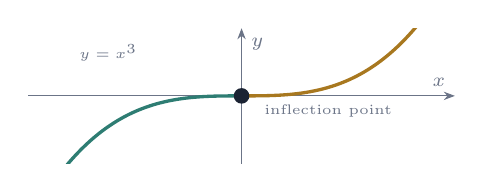
\begin{tikzpicture}\begin{axis}[sem,width=7cm,height=3.3cm,xmin=-1.6,xmax=1.6,ymin=-2.2,ymax=2.2,xtick=\empty,ytick=\empty]
    \addplot[teal,domain=-1.5:0,samples=60]{x^3};\addplot[gold,domain=0:1.5,samples=60]{x^3};
    \addplot[only marks,mark=*,mark size=2.2pt,ink] coordinates{(0,0)};
    \node[muted,font=\tiny,anchor=west] at (axis cs:0.1,-0.5){inflection point};
    \node[muted,font=\tiny] at (axis cs:-1.0,1.4){$y=x^{3}$};
  \end{axis}\end{tikzpicture}\par}
\end{frame}

% ================================================================ example 2
\begin{frame}[t]{Example 2 \ilink{e2}}
  \stmt{Consider the graphs of $y=f'(x)$ and $y=f''(x)$. Determine: 1.\ the intervals on which $f$ is concave up; 2.\ the intervals on which $f$ is concave down; 3.\ the $x$-coordinates of all inflection points of $f(x)$ (if any).}
  \begin{columns}[T]
  \begin{column}{0.48\textwidth}\centering
    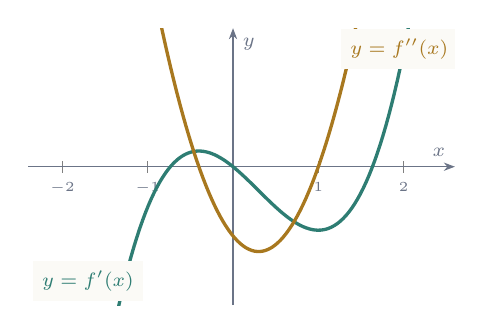
\begin{tikzpicture}\begin{axis}[sem,width=7cm,height=5.1cm,xmin=-2.4,xmax=2.6,ymin=-4,ymax=4,
        xtick={-2,-1,1,2},ytick=\empty]
      \addplot[teal,domain=-2.4:2.6,samples=150]{5*x^3/3-1.5*x^2-2*x};
      \addplot[gold,domain=-2.4:2.6,samples=150]{5*x^2-3*x-2};
      \node[teal,font=\scriptsize,fill=bg] at (axis cs:-1.7,-3.3){$y=f'(x)$};
      \node[gold,font=\scriptsize,fill=bg] at (axis cs:1.95,3.4){$y=f''(x)$};
    \end{axis}\end{tikzpicture}\par
    {\tiny\color{muted} graphs redrawn with the same zeros of $f''$ as Figure 4.2.7}
  \end{column}
  \begin{column}{0.48\textwidth}\small
    {\color{gold}\bfseries\underline{Solution}}\par\vspace{0.15cm}
    Using the graphs and the test for concavity:\par\vspace{0.2cm}
    \uncover<2->{1.\ $f$ is concave up on $\left(-\infty,-\tfrac25\right),\ (1,\infty)$\par\vspace{0.25cm}}
    \uncover<3->{2.\ $f$ is concave down on $\left(-\tfrac25,1\right)$\par\vspace{0.25cm}}
    \uncover<4->{3.\ Inflection points of $f$ occur at\par\centering $\boxed{x=-\tfrac25\ \text{and}\ x=1}$}
  \end{column}
  \end{columns}
\end{frame}

% ================================================================ examples 3,6,8,9
\begin{frame}[t]{Example 3 \ilink{e3}}
\stmt{For $f(x)=x^{3}-6x^{2}+9x+30$, find the intervals on which $f$ is concave up or down, and find all inflection points (if any).}
\sol
\only<1-5>{%
\vspace{0.1cm}{\small{\centering$\renewcommand{\arraystretch}{1.3}\begin{array}{@{}>{\displaystyle}r@{}>{\displaystyle}l@{}}
\multicolumn{2}{@{}l@{}}{\uncover<1->{\parbox[t]{12cm}{\raggedright \alt<1>{}{\color{dimc}}\hspace*{\textleft}$f$ is a polynomial: defined for all $x\in\mathbb{R}$}}}\\[4pt]
\uncover<2->{\alt<2>{}{\color{dimc}} f'(x) } &\uncover<2->{\alt<2>{}{\color{dimc}} {}= 3x^{2}-12x+9}\\[7pt]
\uncover<3->{\alt<3>{}{\color{dimc}} f''(x) } &\uncover<3->{\alt<3>{}{\color{dimc}} {}= 6x-12}\\[7pt]
\uncover<4->{\alt<4>{}{\color{dimc}} 6x-12 } &\uncover<4->{\alt<4>{}{\color{dimc}} {}= 0\;\Longrightarrow\;x=2}\\[7pt]
\multicolumn{2}{@{}l@{}}{\uncover<5->{\parbox[t]{12cm}{\raggedright \alt<5>{}{\color{dimc}}\hspace*{\textleft}Intervals: $(-\infty,2),\ (2,\infty)$}}}\\[4pt]
\end{array}$\par}}}
\only<6->{%
\vspace{0.15cm}\begin{columns}[T]
\begin{column}{0.40\textwidth}\centering
\adjustbox{max width=\linewidth,max totalheight=4.85cm}{\begin{varwidth}{16cm}\small
{\centering$\renewcommand{\arraystretch}{1.3}\begin{array}{@{}>{\displaystyle}r@{}>{\displaystyle}l@{}}
\multicolumn{2}{@{}l@{}}{\parbox[t]{6.6cm}{\raggedright \hspace*{\textleft}$f$ is a polynomial: defined for all $x\in\mathbb{R}$}}\\[4pt]
 f'(x)  & {}= 3x^{2}-12x+9\\[7pt]
 f''(x)  & {}= 6x-12\\[7pt]
 6x-12  & {}= 0\;\Longrightarrow\;x=2\\[7pt]
\multicolumn{2}{@{}l@{}}{\parbox[t]{6.6cm}{\raggedright \hspace*{\textleft}Intervals: $(-\infty,2),\ (2,\infty)$}}\\[4pt]
\end{array}$\par}
\end{varwidth}}\end{column}
\begin{column}{0.01\textwidth}{\color{gold}\vrule height 4.85cm width 0.8pt}\end{column}
\begin{column}{0.56\textwidth}\centering\adjustbox{max width=\linewidth,max totalheight=4.85cm}{\begin{varwidth}{16cm}\small{\centering$\renewcommand{\arraystretch}{1.3}\begin{array}{@{}>{\displaystyle}r@{}>{\displaystyle}l@{}}
\multicolumn{2}{c}{\uncover<6->{\mbox{\alt<6,9->{}{\color{dimc}}{\scriptsize\setlength{\tabcolsep}{6pt}\renewcommand{\arraystretch}{1.25}\begin{tabular}{@{}l|cc@{}}Interval & $(-\infty,2)$ & $(2,\infty)$\\\hline Test value $k$ & $0$ & $3$\\\hline Sign of $f''(k)$ & $-$ & $+$\\\hline Behavior of $f(x)$ & concave downward & concave upward\end{tabular}}}}}\\[6pt]
\multicolumn{2}{@{}l@{}}{\uncover<7->{\parbox[t]{7.4cm}{\raggedright \alt<7,9->{}{\color{dimc}}\hspace*{\textleft}Concave up on $(2,\infty)$, concave down on $(-\infty,2)$}}}\\[4pt]
\uncover<8->{\alt<8,9->{}{\color{dimc}} f(2) } &\uncover<8->{\alt<8,9->{}{\color{dimc}} {}= 32\;\Longrightarrow\;\boxed{(2,\,32)\ \text{is an inflection point}}}\\[7pt]
\end{array}$\par}\end{varwidth}}\end{column}
\end{columns}}
\only<9>{}
\end{frame}

\begin{frame}[t]{Example 3 \textnormal{\small\color{muted}--- graph} \ilink{e3}}
\vspace{0.4cm}\centering
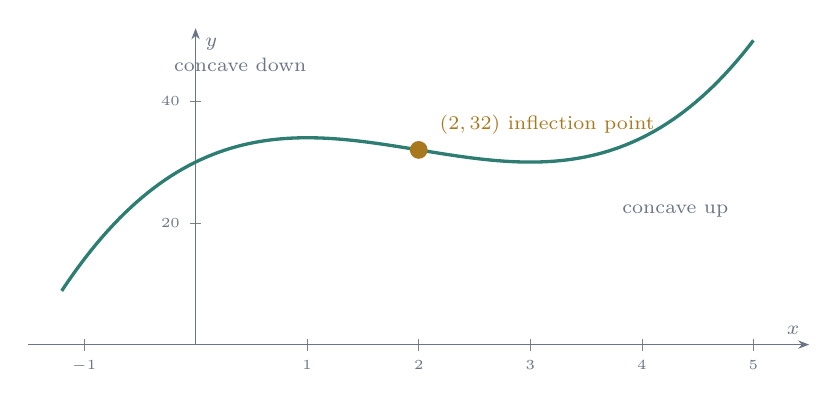
\begin{tikzpicture}\begin{axis}[sem,width=11.5cm,height=5.6cm,xmin=-1.5,xmax=5.5,ymin=0,ymax=52]\addplot[teal,domain=-1.2:5,samples=120]{x^3-6*x^2+9*x+30};\addplot[only marks,mark=*,mark size=2.6pt,gold] coordinates{(2,32)};\node[gold,font=\scriptsize,anchor=south west] at (axis cs:2.1,33){$(2,32)$ inflection point};\node[muted,font=\scriptsize] at (axis cs:0.4,46){concave down};\node[muted,font=\scriptsize] at (axis cs:4.3,22){concave up};\end{axis}\end{tikzpicture}
\end{frame}

\begin{frame}[t]{Example 6 \ilink{e6}}
\stmt{For $f(x)=\dfrac{x+3}{x-5}$, find the intervals on which $f$ is concave up or down, and find all inflection points (if any).}
\sol
\only<1-4>{%
\vspace{0.1cm}{\small{\centering$\renewcommand{\arraystretch}{1.3}\begin{array}{@{}>{\displaystyle}r@{}>{\displaystyle}l@{}}
\multicolumn{2}{@{}l@{}}{\uncover<1->{\parbox[t]{12cm}{\raggedright \alt<1>{}{\color{dimc}}\hspace*{\textleft}$f$ is rational: $D_f=(-\infty,5)\cup(5,\infty)$, twice differentiable at any $x\neq 5$}}}\\[4pt]
\uncover<2->{\alt<2>{}{\color{dimc}} f'(x) } &\uncover<2->{\alt<2>{}{\color{dimc}} {}= \frac{-8}{(x-5)^{2}}}\\[7pt]
\uncover<3->{\alt<3>{}{\color{dimc}} f''(x) } &\uncover<3->{\alt<3>{}{\color{dimc}} {}= \frac{16}{(x-5)^{3}}}\\[7pt]
\multicolumn{2}{@{}l@{}}{\uncover<4->{\parbox[t]{12cm}{\raggedright \alt<4>{}{\color{dimc}}\hspace*{\textleft}$f''(x)\neq 0$, and $(x-5)^{3}=0\Rightarrow x=5$: $f''(x)$ does not exist at $x=5$}}}\\[4pt]
\end{array}$\par}}}
\only<5->{%
\vspace{0.15cm}\begin{columns}[T]
\begin{column}{0.40\textwidth}\centering
\adjustbox{max width=\linewidth,max totalheight=4.85cm}{\begin{varwidth}{16cm}\small
{\centering$\renewcommand{\arraystretch}{1.3}\begin{array}{@{}>{\displaystyle}r@{}>{\displaystyle}l@{}}
\multicolumn{2}{@{}l@{}}{\parbox[t]{6.6cm}{\raggedright \hspace*{\textleft}$f$ is rational: $D_f=(-\infty,5)\cup(5,\infty)$, twice differentiable at any $x\neq 5$}}\\[4pt]
 f'(x)  & {}= \frac{-8}{(x-5)^{2}}\\[7pt]
 f''(x)  & {}= \frac{16}{(x-5)^{3}}\\[7pt]
\multicolumn{2}{@{}l@{}}{\parbox[t]{6.6cm}{\raggedright \hspace*{\textleft}$f''(x)\neq 0$, and $(x-5)^{3}=0\Rightarrow x=5$: $f''(x)$ does not exist at $x=5$}}\\[4pt]
\end{array}$\par}
\end{varwidth}}\end{column}
\begin{column}{0.01\textwidth}{\color{gold}\vrule height 4.85cm width 0.8pt}\end{column}
\begin{column}{0.56\textwidth}\centering\adjustbox{max width=\linewidth,max totalheight=4.85cm}{\begin{varwidth}{16cm}\small{\centering$\renewcommand{\arraystretch}{1.3}\begin{array}{@{}>{\displaystyle}r@{}>{\displaystyle}l@{}}
\multicolumn{2}{c}{\uncover<5->{\mbox{\alt<5,9->{}{\color{dimc}}{\setlength{\tabcolsep}{9pt}\begin{tabular}{@{}lccccc@{}}$x$ & $-\infty$ &  & $5$ &  & $+\infty$\\\hline $f''(x)$ &  & $-$ &  & $+$ & \\ $f(x)$ &  & $\frown$ &  & $\smile$ & \end{tabular}}}}}\\[6pt]
\multicolumn{2}{@{}l@{}}{\uncover<6->{\parbox[t]{7.4cm}{\raggedright \alt<6,9->{}{\color{dimc}}\hspace*{\textleft}Concave up on $(5,\infty)$, concave down on $(-\infty,5)$}}}\\[4pt]
\multicolumn{2}{@{}l@{}}{\uncover<7->{\parbox[t]{7.4cm}{\raggedright \alt<7,9->{}{\color{dimc}}\hspace*{\textleft}\textbf{No inflection points}, although the concavity changes around $x=5$,}}}\\[4pt]
\multicolumn{2}{@{}l@{}}{\uncover<8->{\parbox[t]{7.4cm}{\raggedright \alt<8,9->{}{\color{dimc}}\hspace*{\textleft}because $5\notin D_f$}}}\\[4pt]
\end{array}$\par}\end{varwidth}}\end{column}
\end{columns}}
\only<9>{}
\end{frame}

\begin{frame}[t]{Example 6 \textnormal{\small\color{muted}--- graph} \ilink{e6}}
\vspace{0.4cm}\centering
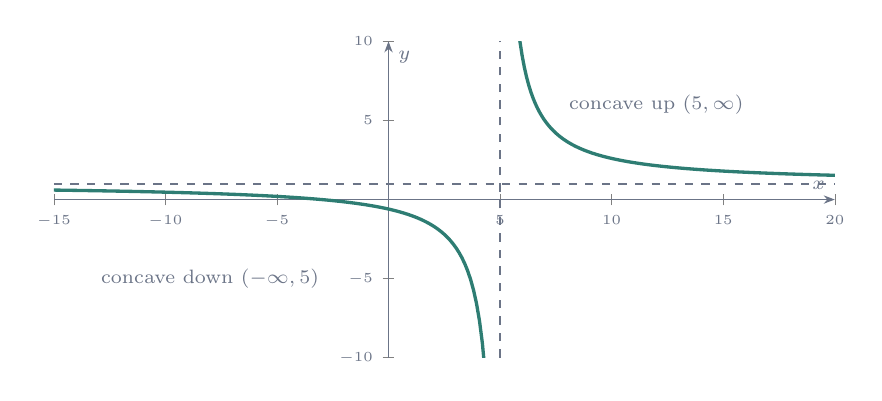
\begin{tikzpicture}\begin{axis}[sem,width=11.5cm,height=5.6cm,xmin=-15,xmax=20,ymin=-10,ymax=10]\addplot[teal,domain=-15:4.6,samples=150]{(x+3)/(x-5)};\addplot[teal,domain=5.4:20,samples=150]{(x+3)/(x-5)};\draw[dashed,muted,line width=0.6pt] (axis cs:5,-10)--(axis cs:5,10);\draw[dashed,muted,line width=0.6pt] (axis cs:-15,1)--(axis cs:20,1);\node[muted,font=\scriptsize] at (axis cs:12,6){concave up $(5,\infty)$};\node[muted,font=\scriptsize] at (axis cs:-8,-5){concave down $(-\infty,5)$};\end{axis}\end{tikzpicture}
\end{frame}

\begin{frame}[t]{Example 8 \ilink{e8}}
\stmt{For $f(x)=x^{2/3}(1-x)$, find the intervals on which $f$ is concave up or down, and find all inflection points (if any).}
\sol
\only<1-5>{%
\vspace{0.1cm}{\small{\centering$\renewcommand{\arraystretch}{1.3}\begin{array}{@{}>{\displaystyle}r@{}>{\displaystyle}l@{}}
\multicolumn{2}{@{}l@{}}{\uncover<1->{\parbox[t]{12cm}{\raggedright \alt<1>{}{\color{dimc}}\hspace*{\textleft}$f$ is a radical function: $D_f=(-\infty,\infty)$, twice differentiable at $x\neq 0$}}}\\[4pt]
\uncover<2->{\alt<2>{}{\color{dimc}} f'(x) } &\uncover<2->{\alt<2>{}{\color{dimc}} {}= \frac{2-5x}{3x^{1/3}}}\\[7pt]
\uncover<3->{\alt<3>{}{\color{dimc}} f''(x) } &\uncover<3->{\alt<3>{}{\color{dimc}} {}= \frac{-2(5x+1)}{9x^{4/3}}}\\[7pt]
\uncover<4->{\alt<4>{}{\color{dimc}} {-}2(5x+1) } &\uncover<4->{\alt<4>{}{\color{dimc}} {}= 0\;\Longrightarrow\;x=-\tfrac{1}{5}\;\Longrightarrow\;f''\!\left(-\tfrac15\right)=0}\\[7pt]
\multicolumn{2}{@{}l@{}}{\uncover<5->{\parbox[t]{12cm}{\raggedright \alt<5>{}{\color{dimc}}\hspace*{\textleft}$f''(x)$ does not exist at $x=0$}}}\\[4pt]
\end{array}$\par}}}
\only<6->{%
\vspace{0.15cm}\begin{columns}[T]
\begin{column}{0.40\textwidth}\centering
\adjustbox{max width=\linewidth,max totalheight=4.85cm}{\begin{varwidth}{16cm}\small
{\centering$\renewcommand{\arraystretch}{1.3}\begin{array}{@{}>{\displaystyle}r@{}>{\displaystyle}l@{}}
\multicolumn{2}{@{}l@{}}{\parbox[t]{6.6cm}{\raggedright \hspace*{\textleft}$f$ is a radical function: $D_f=(-\infty,\infty)$, twice differentiable at $x\neq 0$}}\\[4pt]
 f'(x)  & {}= \frac{2-5x}{3x^{1/3}}\\[7pt]
 f''(x)  & {}= \frac{-2(5x+1)}{9x^{4/3}}\\[7pt]
 {-}2(5x+1)  & {}= 0\;\Longrightarrow\;x=-\tfrac{1}{5}\;\Longrightarrow\;f''\!\left(-\tfrac15\right)=0\\[7pt]
\multicolumn{2}{@{}l@{}}{\parbox[t]{6.6cm}{\raggedright \hspace*{\textleft}$f''(x)$ does not exist at $x=0$}}\\[4pt]
\end{array}$\par}
\end{varwidth}}\end{column}
\begin{column}{0.01\textwidth}{\color{gold}\vrule height 4.85cm width 0.8pt}\end{column}
\begin{column}{0.56\textwidth}\centering\adjustbox{max width=\linewidth,max totalheight=4.85cm}{\begin{varwidth}{16cm}\small{\centering$\renewcommand{\arraystretch}{1.3}\begin{array}{@{}>{\displaystyle}r@{}>{\displaystyle}l@{}}
\multicolumn{2}{c}{\uncover<6->{\mbox{\alt<6,11->{}{\color{dimc}}{\setlength{\tabcolsep}{9pt}\begin{tabular}{@{}lccccccc@{}}$x$ & $-\infty$ &  & $-\tfrac15$ &  & $0$ &  & $+\infty$\\\hline $f''(x)$ &  & $+$ &  & $-$ &  & $-$ & \\ $f(x)$ &  & $\smile$ &  & $\frown$ &  & $\frown$ & \end{tabular}}}}}\\[6pt]
\multicolumn{2}{@{}l@{}}{\uncover<7->{\parbox[t]{7.4cm}{\raggedright \alt<7,11->{}{\color{dimc}}\hspace*{\textleft}Concave up on $\left(-\infty,-\tfrac15\right)$; concave down on $\left(-\tfrac15,0\right),\,(0,\infty)$}}}\\[4pt]
\multicolumn{2}{@{}l@{}}{\uncover<8->{\parbox[t]{7.4cm}{\raggedright \alt<8,11->{}{\color{dimc}}\hspace*{\textleft}$f''$ does not change sign around $x=0$: no inflection at $x=0$}}}\\[4pt]
\multicolumn{2}{@{}l@{}}{\uncover<9->{\parbox[t]{7.4cm}{\raggedright \alt<9,11->{}{\color{dimc}}\hspace*{\textleft}$f''$ changes sign around $x=-\tfrac15$ (positive to negative):}}}\\[4pt]
\uncover<10->{\alt<10,11->{}{\color{dimc}} \text{only inflection point} } &\uncover<10->{\alt<10,11->{}{\color{dimc}} {}= \boxed{\left(-\tfrac{1}{5},\ \tfrac{6}{5}\sqrt[3]{\tfrac{1}{25}}\right)}}\\[7pt]
\end{array}$\par}\end{varwidth}}\end{column}
\end{columns}}
\only<11>{}
\end{frame}

\begin{frame}[t]{Example 8 \textnormal{\small\color{muted}--- graph} \ilink{e8}}
\vspace{0.4cm}\centering
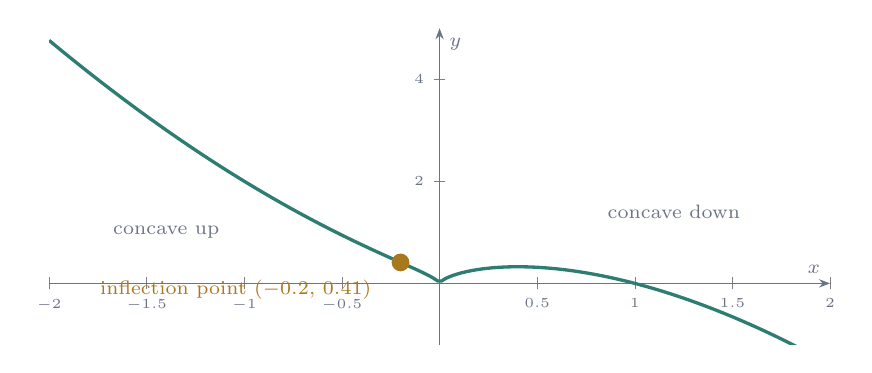
\begin{tikzpicture}\begin{axis}[sem,width=11.5cm,height=5.6cm,xmin=-2,xmax=2,ymin=-1.2,ymax=5]\addplot[teal,domain=-2:2,samples=200]{(x^2)^(1/3)*(1-x)};\addplot[only marks,mark=*,mark size=2.6pt,gold] coordinates{(-0.2,0.4104)};\node[gold,font=\scriptsize,anchor=north east] at (axis cs:-0.3,0.25){inflection point $(-0.2,\,0.41)$};\node[muted,font=\scriptsize] at (axis cs:-1.4,1.0){concave up};\node[muted,font=\scriptsize] at (axis cs:1.2,1.4){concave down};\end{axis}\end{tikzpicture}
\end{frame}

\begin{frame}[t]{Example 9 \ilink{e9}}
\stmt{For $f(x)=x+\sin x,\ x\in[0,2\pi]$, find the intervals on which $f$ is concave up or down, and find all inflection points (if any).}
\sol
\only<1-4>{%
\vspace{0.1cm}{\small{\centering$\renewcommand{\arraystretch}{1.3}\begin{array}{@{}>{\displaystyle}r@{}>{\displaystyle}l@{}}
\multicolumn{2}{@{}l@{}}{\uncover<1->{\parbox[t]{12cm}{\raggedright \alt<1>{}{\color{dimc}}\hspace*{\textleft}$f$ is continuous and twice differentiable on $[0,2\pi]$}}}\\[4pt]
\uncover<2->{\alt<2>{}{\color{dimc}} f'(x) } &\uncover<2->{\alt<2>{}{\color{dimc}} {}= 1+\cos x}\\[7pt]
\uncover<3->{\alt<3>{}{\color{dimc}} f''(x) } &\uncover<3->{\alt<3>{}{\color{dimc}} {}= -\sin x}\\[7pt]
\uncover<4->{\alt<4>{}{\color{dimc}} f''(x) } &\uncover<4->{\alt<4>{}{\color{dimc}} {}= 0\;\Longrightarrow\;x=\pi}\\[7pt]
\end{array}$\par}}}
\only<5->{%
\vspace{0.15cm}\begin{columns}[T]
\begin{column}{0.40\textwidth}\centering
\adjustbox{max width=\linewidth,max totalheight=4.85cm}{\begin{varwidth}{16cm}\small
{\centering$\renewcommand{\arraystretch}{1.3}\begin{array}{@{}>{\displaystyle}r@{}>{\displaystyle}l@{}}
\multicolumn{2}{@{}l@{}}{\parbox[t]{6.6cm}{\raggedright \hspace*{\textleft}$f$ is continuous and twice differentiable on $[0,2\pi]$}}\\[4pt]
 f'(x)  & {}= 1+\cos x\\[7pt]
 f''(x)  & {}= -\sin x\\[7pt]
 f''(x)  & {}= 0\;\Longrightarrow\;x=\pi\\[7pt]
\end{array}$\par}
\end{varwidth}}\end{column}
\begin{column}{0.01\textwidth}{\color{gold}\vrule height 4.85cm width 0.8pt}\end{column}
\begin{column}{0.56\textwidth}\centering\adjustbox{max width=\linewidth,max totalheight=4.85cm}{\begin{varwidth}{16cm}\small{\centering$\renewcommand{\arraystretch}{1.3}\begin{array}{@{}>{\displaystyle}r@{}>{\displaystyle}l@{}}
\multicolumn{2}{c}{\uncover<5->{\mbox{\alt<5,8->{}{\color{dimc}}{\setlength{\tabcolsep}{9pt}\begin{tabular}{@{}lccccc@{}}$x$ & $0$ &  & $\pi$ &  & $2\pi$\\\hline $f''(x)$ &  & $-$ &  & $+$ & \\ $f(x)$ &  & $\frown$ &  & $\smile$ & \end{tabular}}}}}\\[6pt]
\multicolumn{2}{@{}l@{}}{\uncover<6->{\parbox[t]{7.4cm}{\raggedright \alt<6,8->{}{\color{dimc}}\hspace*{\textleft}Concave up on $(\pi,2\pi)$, concave down on $(0,\pi)$}}}\\[4pt]
\uncover<7->{\alt<7,8->{}{\color{dimc}} (\pi,f(\pi)) } &\uncover<7->{\alt<7,8->{}{\color{dimc}} {}= \boxed{(\pi,\,\pi)}\ \text{is the only inflection point}}\\[7pt]
\end{array}$\par}\end{varwidth}}\end{column}
\end{columns}}
\only<8>{}
\end{frame}

\begin{frame}[t]{Example 9 \textnormal{\small\color{muted}--- graph} \ilink{e9}}
\vspace{0.4cm}\centering
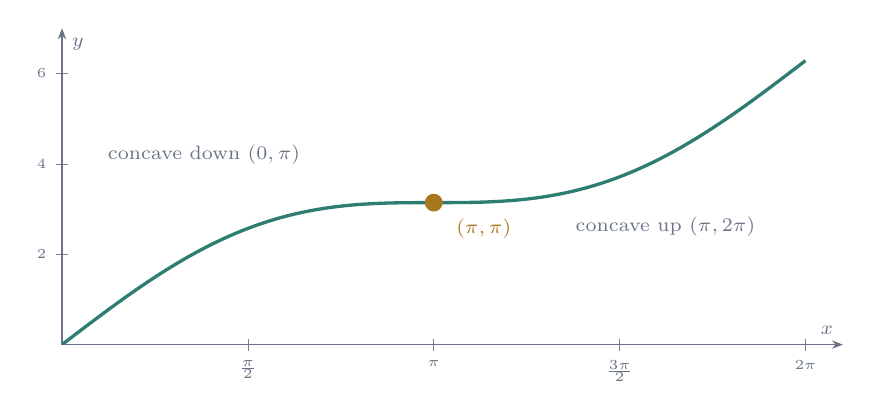
\begin{tikzpicture}\begin{axis}[sem,width=11.5cm,height=5.6cm,xmin=0,xmax=6.6,ymin=0,ymax=7,xtick={0,1.5708,3.1416,4.7124,6.2832},xticklabels={$0$,$\frac{\pi}{2}$,$\pi$,$\frac{3\pi}{2}$,$2\pi$}]\addplot[teal,domain=0:6.2832,samples=150]{x+sin(deg(x))};\addplot[only marks,mark=*,mark size=2.6pt,gold] coordinates{(3.1416,3.1416)};\node[gold,font=\scriptsize,anchor=north west] at (axis cs:3.25,3.0){$(\pi,\pi)$};\node[muted,font=\scriptsize] at (axis cs:1.2,4.2){concave down $(0,\pi)$};\node[muted,font=\scriptsize] at (axis cs:5.1,2.6){concave up $(\pi,2\pi)$};\end{axis}\end{tikzpicture}
\end{frame}

% ================================================================ second derivative test
\begin{frame}[t]{Theorem 4.2.3 \ (The Second Derivative Test)}
  \vspace{0.2cm}
  \begin{block}{Theorem 4.2.3}
    Suppose $f''$ is continuous on an open interval containing $c$ with $f'(c)=0$.
    \begin{itemize}
      \item If $f''(c)>0$, then $f$ has a relative minimum at $c$.
      \item If $f''(c)<0$, then $f$ has a relative maximum at $c$.
      \item If $f''(c)=0$, then the test is inconclusive; $f$ may have a relative maximum, relative minimum, or neither at $c$.
    \end{itemize}
  \end{block}
  \small\vspace{0.1cm}
  In such cases ($f''(c)=0$), we may use the first derivative test.
\end{frame}

% ================================================================ example 10(1), challenging, communicate
\begin{frame}[t]{Example 10 (1) \textnormal{\small\color{muted}--- relative extrema} \ilink{e10}}
\stmt{Find the relative extrema of $f$ using the second derivative test if applicable. Discuss the concavity of $f$ and find the point(s) of inflection: \ $f(x)=3x^{4}-4x^{3}-6x^{2}+12x+1,\ [-2,2]$.}
\sol
\only<1-6>{%
\vspace{0.1cm}{\small{\centering$\renewcommand{\arraystretch}{1.3}\begin{array}{@{}>{\displaystyle}r@{}>{\displaystyle}l@{}}
\uncover<1->{\alt<1>{}{\color{dimc}} f'(x) } &\uncover<1->{\alt<1>{}{\color{dimc}} {}= 12x^{3}-12x^{2}-12x+12}\\[7pt]
\uncover<2->{\alt<2>{}{\color{dimc}} f''(x) } &\uncover<2->{\alt<2>{}{\color{dimc}} {}= 36x^{2}-24x-12}\\[7pt]
\uncover<3->{\alt<3>{}{\color{dimc}} \Longrightarrow\;f''(x) } &\uncover<3->{\alt<3>{}{\color{dimc}} {}= 12(3x^{2}-2x-1)}\\[7pt]
\uncover<4->{\alt<4>{}{\color{dimc}} 12x^{3}-12x^{2}-12x+12 } &\uncover<4->{\alt<4>{}{\color{dimc}} {}= 0}\\[7pt]
\uncover<5->{\alt<5>{}{\color{dimc}} 12(x^{3}-x^{2}-x+1) } &\uncover<5->{\alt<5>{}{\color{dimc}} {}= 0}\\[7pt]
\uncover<6->{\alt<6>{}{\color{dimc}} 12\left[x^{2}(x-1)-(x-1)\right] } &\uncover<6->{\alt<6>{}{\color{dimc}} {}= 0}\\[7pt]
\end{array}$\par}}}
\only<7->{%
\vspace{0.15cm}\begin{columns}[T]
\begin{column}{0.40\textwidth}\centering
\adjustbox{max width=\linewidth,max totalheight=4.85cm}{\begin{varwidth}{16cm}\small
{\centering$\renewcommand{\arraystretch}{1.3}\begin{array}{@{}>{\displaystyle}r@{}>{\displaystyle}l@{}}
 f'(x)  & {}= 12x^{3}-12x^{2}-12x+12\\[7pt]
 f''(x)  & {}= 36x^{2}-24x-12\\[7pt]
 \Longrightarrow\;f''(x)  & {}= 12(3x^{2}-2x-1)\\[7pt]
 12x^{3}-12x^{2}-12x+12  & {}= 0\\[7pt]
 12(x^{3}-x^{2}-x+1)  & {}= 0\\[7pt]
 12\left[x^{2}(x-1)-(x-1)\right]  & {}= 0\\[7pt]
\end{array}$\par}
\end{varwidth}}\end{column}
\begin{column}{0.01\textwidth}{\color{gold}\vrule height 4.85cm width 0.8pt}\end{column}
\begin{column}{0.56\textwidth}\centering\adjustbox{max width=\linewidth,max totalheight=4.85cm}{\begin{varwidth}{16cm}\small{\centering$\renewcommand{\arraystretch}{1.3}\begin{array}{@{}>{\displaystyle}r@{}>{\displaystyle}l@{}}
\uncover<7->{\alt<7,14->{}{\color{dimc}} 12(x-1)(x^{2}-1) } &\uncover<7->{\alt<7,14->{}{\color{dimc}} {}= 0}\\[7pt]
\uncover<8->{\alt<8,14->{}{\color{dimc}} 12(x+1)(x-1)^{2} } &\uncover<8->{\alt<8,14->{}{\color{dimc}} {}= 0\;\Longrightarrow\;x=-1,\ x=1}\\[7pt]
\uncover<9->{\alt<9,14->{}{\color{dimc}} f''(-1) } &\uncover<9->{\alt<9,14->{}{\color{dimc}} {}= 48>0,\quad f''(1)=0}\\[7pt]
\multicolumn{2}{@{}l@{}}{\uncover<10->{\parbox[t]{7.4cm}{\raggedright \alt<10,14->{}{\color{dimc}}\hspace*{\textleft}By the Second Derivative Test: \textbf{relative minimum at $x=-1$}}}}\\[4pt]
\multicolumn{2}{@{}l@{}}{\uncover<11->{\parbox[t]{7.4cm}{\raggedright \alt<11,14->{}{\color{dimc}}\hspace*{\textleft}At $x=1$: test inconclusive; $f'$ does not change sign at $x=1$:}}}\\[4pt]
\uncover<12->{\alt<12,14->{}{\color{dimc}} f'(0.5) } &\uncover<12->{\alt<12,14->{}{\color{dimc}} {}= 4.5>0,\quad f'(1.5)=\tfrac{15}{2}>0}\\[7pt]
\multicolumn{2}{@{}l@{}}{\uncover<13->{\parbox[t]{7.4cm}{\raggedright \alt<13,14->{}{\color{dimc}}\hspace*{\textleft}$\Longrightarrow$ no relative maximum or minimum at $x=1$}}}\\[4pt]
\end{array}$\par}\end{varwidth}}\end{column}
\end{columns}}
\only<14>{}
\end{frame}

\begin{frame}[t]{Example 10 (1) \textnormal{\small\color{muted}--- concavity} \ilink{e10}}
\stmt{$f(x)=3x^{4}-4x^{3}-6x^{2}+12x+1,\ [-2,2]$, \quad $f''(x)=12(3x^{2}-2x-1)$.}
\sol
\only<1->{%
\vspace{0.1cm}{\small{\centering$\renewcommand{\arraystretch}{1.3}\begin{array}{@{}>{\displaystyle}r@{}>{\displaystyle}l@{}}
\uncover<1->{\alt<1,7->{}{\color{dimc}} f''(x) } &\uncover<1->{\alt<1,7->{}{\color{dimc}} {}= 0\;\text{if}\;3x^{2}-2x-1=0}\\[7pt]
\uncover<2->{\alt<2,7->{}{\color{dimc}} (3x+1)(x-1) } &\uncover<2->{\alt<2,7->{}{\color{dimc}} {}= 0\;\Longrightarrow\;x=-\tfrac13\ \text{or}\ x=1}\\[7pt]
\multicolumn{2}{@{}l@{}}{\uncover<3->{\parbox[t]{12cm}{\raggedright \alt<3,7->{}{\color{dimc}}\hspace*{\textleft}Intervals: $\left(-2,-\tfrac13\right),\ \left(-\tfrac13,1\right),\ (1,2)$}}}\\[4pt]
\multicolumn{2}{c}{\uncover<4->{\mbox{\alt<4,7->{}{\color{dimc}}{\scriptsize\setlength{\tabcolsep}{6pt}\renewcommand{\arraystretch}{1.25}\begin{tabular}{@{}l|ccc@{}}Interval & $\left(-2,-\tfrac13\right)$ & $\left(-\tfrac13,1\right)$ & $(1,2)$\\\hline Test value $k$ & $-1$ & $0$ & $1.5$\\\hline Sign of $f''(k)$ & $+$ & $-$ & $+$\\\hline Behavior of $f(x)$ & concave upward & concave downward & concave upward\end{tabular}}}}}\\[6pt]
\multicolumn{2}{@{}l@{}}{\uncover<5->{\parbox[t]{12cm}{\raggedright \alt<5,7->{}{\color{dimc}}\hspace*{\textleft}Concavity changes at $x=-\tfrac13$ and $x=1$:}}}\\[4pt]
\uncover<6->{\alt<6,7->{}{\color{dimc}} \text{inflection points} } &\uncover<6->{\alt<6,7->{}{\color{dimc}} {}= \boxed{\left(-\tfrac13,\,-\tfrac{94}{27}\right)},\ \boxed{(1,\,6)}}\\[7pt]
\end{array}$\par}}}
\only<7>{}
\end{frame}

\begin{frame}[t]{Example 10 (1) \textnormal{\small\color{muted}--- graph} \ilink{e10}}
\vspace{0.4cm}\centering
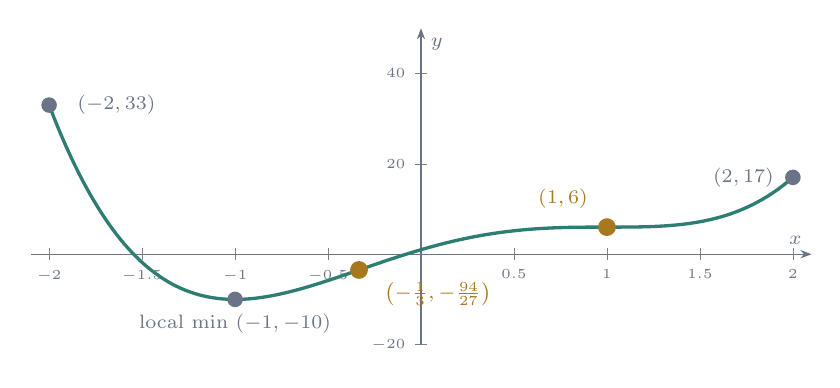
\begin{tikzpicture}\begin{axis}[sem,width=11.5cm,height=5.6cm,xmin=-2.1,xmax=2.1,ymin=-20,ymax=50]\addplot[teal,domain=-2:2,samples=200]{3*x^4-4*x^3-6*x^2+12*x+1};\addplot[only marks,mark=*,mark size=2.6pt,gold] coordinates{(-0.3333,-3.4815)(1,6)};\addplot[only marks,mark=*,mark size=2.2pt,muted] coordinates{(-1,-10)(-2,33)(2,17)};\node[gold,font=\scriptsize,anchor=north west] at (axis cs:-0.25,-4){$\left(-\frac13,-\frac{94}{27}\right)$};\node[gold,font=\scriptsize,anchor=south east] at (axis cs:0.95,8){$(1,6)$};\node[muted,font=\scriptsize,anchor=north] at (axis cs:-1,-11){local min $(-1,-10)$};\node[muted,font=\scriptsize,anchor=west] at (axis cs:-1.9,33){$(-2,33)$};\node[muted,font=\scriptsize,anchor=east] at (axis cs:1.95,17){$(2,17)$};\end{axis}\end{tikzpicture}
\end{frame}

\begin{frame}[t]{Challenging Problems 5}
\stmt{Suppose $f$ and $g$ are both concave up on $(-\infty,\infty)$. Under what condition on $f$ will the composite function $h(x)=f(g(x))$ be concave up?}
\sol
\only<1-5>{%
\vspace{0.1cm}{\small{\centering$\renewcommand{\arraystretch}{1.3}\begin{array}{@{}>{\displaystyle}r@{}>{\displaystyle}l@{}}
\multicolumn{2}{@{}l@{}}{\uncover<1->{\parbox[t]{12cm}{\raggedright \alt<1>{}{\color{dimc}}\hspace*{\textleft}(Assume $f,g$ twice differentiable.)}}}\\[4pt]
\uncover<2->{\alt<2>{}{\color{dimc}} h'(x) } &\uncover<2->{\alt<2>{}{\color{dimc}} {}= f'(g(x))\,g'(x)}\\[7pt]
\uncover<3->{\alt<3>{}{\color{dimc}} h''(x) } &\uncover<3->{\alt<3>{}{\color{dimc}} {}= f''(g(x))\,[g'(x)]^{2}+f'(g(x))\,g''(x)}\\[7pt]
\multicolumn{2}{@{}l@{}}{\uncover<4->{\parbox[t]{12cm}{\raggedright \alt<4>{}{\color{dimc}}\hspace*{\textleft}$f''>0$, $[g']^{2}\geq 0$ $\Longrightarrow$ first term $\geq 0$; \ $g''>0$}}}\\[4pt]
\multicolumn{2}{@{}l@{}}{\uncover<5->{\parbox[t]{12cm}{\raggedright \alt<5>{}{\color{dimc}}\hspace*{\textleft}$\Longrightarrow\ h''(x)>0$ whenever $f'(g(x))>0$}}}\\[4pt]
\end{array}$\par}}}
\only<6->{%
\vspace{0.15cm}\begin{columns}[T]
\begin{column}{0.40\textwidth}\centering
\adjustbox{max width=\linewidth,max totalheight=4.85cm}{\begin{varwidth}{16cm}\small
{\centering$\renewcommand{\arraystretch}{1.3}\begin{array}{@{}>{\displaystyle}r@{}>{\displaystyle}l@{}}
\multicolumn{2}{@{}l@{}}{\parbox[t]{6.6cm}{\raggedright \hspace*{\textleft}(Assume $f,g$ twice differentiable.)}}\\[4pt]
 h'(x)  & {}= f'(g(x))\,g'(x)\\[7pt]
 h''(x)  & {}= f''(g(x))\,[g'(x)]^{2}+f'(g(x))\,g''(x)\\[7pt]
\multicolumn{2}{@{}l@{}}{\parbox[t]{6.6cm}{\raggedright \hspace*{\textleft}$f''>0$, $[g']^{2}\geq 0$ $\Longrightarrow$ first term $\geq 0$; \ $g''>0$}}\\[4pt]
\multicolumn{2}{@{}l@{}}{\parbox[t]{6.6cm}{\raggedright \hspace*{\textleft}$\Longrightarrow\ h''(x)>0$ whenever $f'(g(x))>0$}}\\[4pt]
\end{array}$\par}
\end{varwidth}}\end{column}
\begin{column}{0.01\textwidth}{\color{gold}\vrule height 4.85cm width 0.8pt}\end{column}
\begin{column}{0.56\textwidth}\centering\adjustbox{max width=\linewidth,max totalheight=4.85cm}{\begin{varwidth}{16cm}\small{\centering$\renewcommand{\arraystretch}{1.3}\begin{array}{@{}>{\displaystyle}r@{}>{\displaystyle}l@{}}
\multicolumn{2}{@{}l@{}}{\uncover<6->{\parbox[t]{7.4cm}{\raggedright \alt<6,11->{}{\color{dimc}}\hspace*{\textleft}\textbf{Condition:} $f$ increasing ($f'>0$) $\Longrightarrow$ $h=f\circ g$ is concave up}}}\\[4pt]
\multicolumn{2}{@{}l@{}}{\uncover<7->{\parbox[t]{7.4cm}{\raggedright \alt<7,11->{}{\color{dimc}}\hspace*{\textleft}Without it, it may fail: $f(u)=e^{-u}$ (concave up, decreasing),}}}\\[4pt]
\uncover<8->{\alt<8,11->{}{\color{dimc}} g(x) } &\uncover<8->{\alt<8,11->{}{\color{dimc}} {}= x^{2}\;\Longrightarrow\;h(x)=e^{-x^{2}}}\\[7pt]
\uncover<9->{\alt<9,11->{}{\color{dimc}} h''(x) } &\uncover<9->{\alt<9,11->{}{\color{dimc}} {}= (4x^{2}-2)e^{-x^{2}},\quad h''(0)=-2<0}\\[7pt]
\multicolumn{2}{@{}l@{}}{\uncover<10->{\parbox[t]{7.4cm}{\raggedright \alt<10,11->{}{\color{dimc}}\hspace*{\textleft}$\Longrightarrow$ $h$ is concave down near $0$}}}\\[4pt]
\end{array}$\par}\end{varwidth}}\end{column}
\end{columns}}
\only<11>{}
\end{frame}

\begin{frame}[t]{Communicate with Mathematics 2}
\stmt{Prove that a quadratic function $f(x)=ax^{2}+bx+c$ has no inflection points.}
\sol
\only<1->{%
\vspace{0.1cm}{\small{\centering$\renewcommand{\arraystretch}{1.3}\begin{array}{@{}>{\displaystyle}r@{}>{\displaystyle}l@{}}
\multicolumn{2}{@{}l@{}}{\uncover<1->{\parbox[t]{12cm}{\raggedright \alt<1,8->{}{\color{dimc}}\hspace*{\textleft}$f$ is quadratic $\Longrightarrow a\neq 0$}}}\\[4pt]
\uncover<2->{\alt<2,8->{}{\color{dimc}} f'(x) } &\uncover<2->{\alt<2,8->{}{\color{dimc}} {}= 2ax+b}\\[7pt]
\uncover<3->{\alt<3,8->{}{\color{dimc}} f''(x) } &\uncover<3->{\alt<3,8->{}{\color{dimc}} {}= 2a\neq 0\quad\text{for all } x}\\[7pt]
\multicolumn{2}{@{}l@{}}{\uncover<4->{\parbox[t]{12cm}{\raggedright \alt<4,8->{}{\color{dimc}}\hspace*{\textleft}$f''$ exists everywhere and is never $0$:}}}\\[4pt]
\multicolumn{2}{@{}l@{}}{\uncover<5->{\parbox[t]{12cm}{\raggedright \alt<5,8->{}{\color{dimc}}\hspace*{\textleft}by Theorem 4.2.2 there is no candidate $c$ with $f''(c)=0$ or $f''(c)$ undefined}}}\\[4pt]
\multicolumn{2}{@{}l@{}}{\uncover<6->{\parbox[t]{12cm}{\raggedright \alt<6,8->{}{\color{dimc}}\hspace*{\textleft}($a>0$: concave up on $\mathbb{R}$; \ $a<0$: concave down on $\mathbb{R}$)}}}\\[4pt]
\multicolumn{2}{@{}l@{}}{\uncover<7->{\parbox[t]{12cm}{\raggedright \alt<7,8->{}{\color{dimc}}\hspace*{\textleft}$\Longrightarrow$ \textbf{$f$ has no inflection points} \hfill $\blacksquare$}}}\\[4pt]
\end{array}$\par}}}
\only<8>{}
\end{frame}

% ================================================================ closing
{\setbeamertemplate{footline}{}
\begin{frame}[plain]
  \centering\vspace*{2.2cm}
  {\fontsize{28}{34}\selectfont\bfseries Thank you}\par\vspace{0.2cm}
  {\color{gold}\rule{4.5cm}{1.2pt}}\par\vspace{0.25cm}
  {\color{gold}\large Questions \& discussion}\par\vspace{0.3cm}
  {\color{muted}\small Dr.\ Wessam Gouda \;$\cdot$\; Section 4.2 --- Concavity and Inflection Points}
\end{frame}}

\end{document}
